\chapter{Background}
\label{cha:bkg}

%\textcolor{red}{I'd love to REWRITE it.}
%
%
%\section{How Vision is Presented in the Brain}
%\label{sec:bio}
%
%\begin{figure}
%	\centering
%	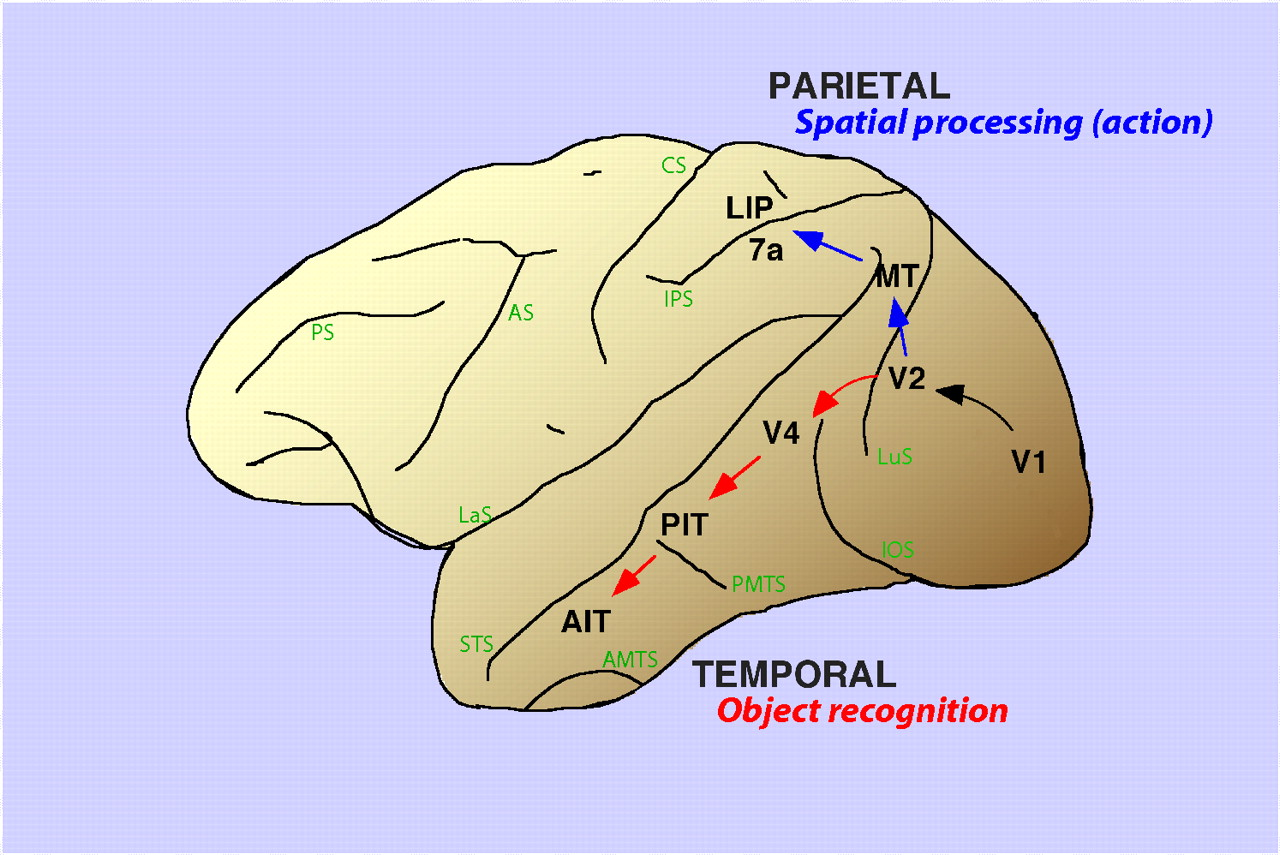
\includegraphics[width=0.8\textwidth]{pics_report/twoPaths.jpg}
%	\caption{The dorsal and ventral pathway in the brain~\cite{lehky2007comparison}.
%	The dorsal stream (blue) arrives to the parietal lobe, whereas the ventral pathway (red) reaches the inferotemporal (IT) cortex in the temporal lobe.}
%	\label{Fig:TwoPath}
%\end{figure}
%The central visual system consists of several cortical areas responsible for visual processing, which are placed in a hierarchical pattern according to the anatomical experiments~\cite{felleman1991distributed}.
%There are two basic streams locating in the visual area: a dorsal and a ventral pathway (Figure~\ref{Fig:TwoPath}).
%
%They differ in behavioural patterns according to the observation from brain lesions~\cite{prado2005two}, and also in functions where the dorsal pathway targets on the `where' tasks and the ventral on the `what'.
%The ventral visual stream holds the critical circuits for object recognition and stimulus identification, whereas the dorsal pathway pathway contributes to the processing of the spatial location of the stimulus~\cite{prado2005two, Ungerleider1994157}.
%Another definition of the difference between these two pathways is a `perception/action' dichotomy: the ventral (`perception') stream perceives the world by means of object recognition and memory, while the dorsal (`action') stream provides real-time visual guidance for motor actions such as eye movements and grasping objects~\cite{goodale1992separate}. 
%
%This research mainly focuses on the ventral visual pathway, since it dominates the object recognition among the cortical areas.
%Thus, the dorsal pathway will beyond the scope of the this study. 
%
%
%\subsection{Cortical Areas in The Ventral Visual Pathway}
%The ventral visual pathway starts from the primary visual cortex V1 in the occipital cortex through areas such as V2 and V4 to the Inferotemporal (IT) cortex.
%These cortex areas are divided based on the anatomical experiments and retinotopic maps.
%Accordingly, the IT complex is commonly parsed into sub areas such as TEO and TE~\cite{janssen2000selectivity,von1947neocortex} or posterior IT (PIT), central IT (CIT), and anterior IT (AIT)~\cite{felleman1991distributed}.
%\subsubsection{Primary Visual Cortex: V1}
%As the simplest and earliest cortical area in the ventral stream, the primary visual cortex V1 is the best-studied since the well-known discovery of the orientation selectivity by Hubel and Wiesel~\cite{hubel1959receptive} in 1958.
%The retinotopic map is well-defined to transform spatial information from retinal image to V1~\cite{tootell1982deoxyglucose}.
%In human and animals with a fovea in the retina, the central 10 degrees of the visual field occupies roughly half of V1.
%This distorted retinotopic map in V1 is a phenomenon known as cortical magnification.
%
%\begin{figure}
%	\centering
%	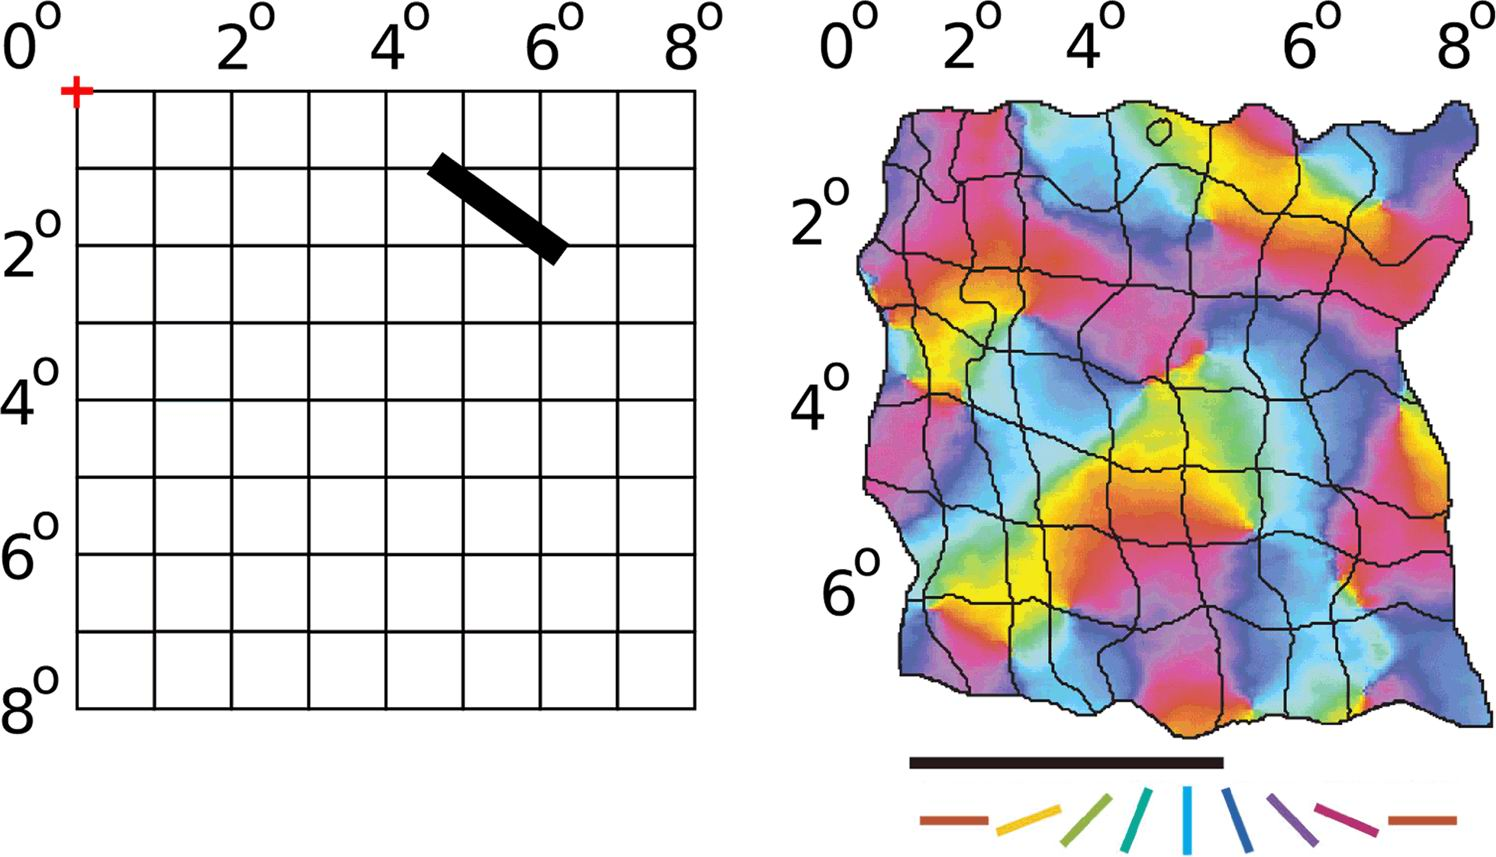
\includegraphics[width=0.8\textwidth]{pics_report/retinotopic.jpg}
%	\caption{The retinotopic and orientation map on the surface of V1 of a tree shrew~\cite{bednar2009topographica}.
%	The visual field (left) with a fixation point marked as a red cross on the up-left corner can be divided into a regular grid.
%	Each square represents a 1$^\circ \times 1^\circ$ area of visual space.
%	In cortical area V1 of mammals, neurons are arranged into a retinotopic map (right) responding to the retinal visual space.
%	As an example, the retinotopic map shows the orientation preference of the V1 neurons of a tree shrew for an 8$^\circ \times 7^\circ$ area of visual space (adapted from~\cite{bosking2002spatial}; scale bar is 1 mm).}
%	\label{Fig:retinotopic}
%\end{figure}
%
%In the spatial domain, V1 neurons are tuned to Gabor-like transforms applied to their small local receptive field.
%The retinotopic and orientation map on the surface of V1 of a tree shrew is shown in Figure~\ref{Fig:retinotopic}.
%A black bar presented in the retinal image evokes a response in the corresponding grid square of V1 (6$^\circ$, 2$^\circ$) depending on the orientation of the stimulus.
%The coloured map on the right represents the preferred orientation of neurons in each location.
%Thus the black bar shown at left will activate V1 neurons coloured in purple in the specific square.
%In theory, these Gabor-like filters together can carry out neuronal processing of spatial frequency, orientation, motion, direction, speed, and many other spatiotemporal features.
%Similar maps could be plotted for this same area showing preference for other visual features.
%
%\subsubsection{Prestriate Cortex: V2}
%Visual area V2, also called prestriate cortex~\cite{an2012distinct}, is the second major area located in the occipital lobe of the primate brain, and the first region within the visual association area~\cite{wu2011early}. 
%It receives strong feed-forward connections from V1 and has many properties in common with V1. 
%
%The responses of V2 neurons are tuned to simple shapes such as orientation and sinusoidal gratings. 
%Moreover, V2 neurons are able to represent variety of higher order shapes that are based on contours (e.g., angles and curves with multiple orientations at different subregions within a single receptive field) or grating patterns~\cite{hegde2000selectivity}.
%The responses of many V2 neurons are also modulated for complex properties: orientation of illusory contours~\cite{anzai2007neurons}, binocular disparity~\cite{daniel2009whither}, and whether the stimulus is part of the figure or the ground~\cite{qiu2005figure}.
%
%%In a recent study, the Layer 6 cells of the V2 cortex were found to play a very important role in the storage of Object Recognition Memory as well as the conversion of short-term object memories into long-term memories.[23]
%
%\subsubsection{Visual Area V4}
%Area V4 is the third cortical area in the ventral stream, receiving strong feedforward input from V2 and transmitting to the PIT.
%It also receives direct inputs from V1 which are mostly generated in the visual central space.
%V4 is the first area in the ventral stream to show strong attentional modulation.
%Most studies indicate that selective attention can change firing rates in V4 by about 20\%~\cite{filipe2013human}.
%This discovery found by Moran and Desimone~\cite{moran1985selective} was the first report of attention effects anywhere in the visual cortex.
%
%Although V4 is mainly modulated for colour recognition, it is also tuned for orientation and spatial frequency similar to V1.
%Comparing to V1, V4 responds to more complex object features with intermediate complexity but is not tuned for complex objects as areas in the inferotemporal cortex are~\cite{williams2007biological}.
%
%\subsubsection{Inferotemporal Cortex: IT}
%Inferotemporal Cortex is only found in the temporal lobe in primates including humans. 
%It is tuned to a range of object features complexity starting with simpler patterns in the PIT/TEO~\cite{tanaka1991coding};
%And the complexity increases along the ventral stream towards AIT/TE where objects are represented and recognised~\cite{dean1976effects}.
%The high-order complex features includes the combinations of colour or texture with complicated shapes~\cite{tanaka1991coding}, and body parts such as faces and hands~\cite{gross2008single}.
%The distinguishing features of the IT cortex is that the neuronal responses are position and size invariant~\cite{schwartz1983shape,logothetis1995psychophysical}, and also invariant to changes in luminance, texture, and relative motion ~\cite{sary1993cue,perry2014feature}.
%It is wide-accepted that the identity-preserving transformation invariance makes IT ideal for representing objects despite changes in the surrounding environment and retinal image.
%
%In the next section, this report will explore the detailed mechanism of object representation in this cortical area.
%%PFC
%\subsection{Object Representation in IT}
%\label{sec:orIT}
%%\subsection{Untangling Object Representation}
%The neuronal representation in the cortical area of IT is considered to be the spatio-temporal pattern of spikes.
%The spiking activities of single neurons and populations are thought to hold the key to encode visual information.
%In Section~\ref{sec:SNNintro}, the report will introduce single neuron models and spike coding mechanisms in computational spiking neural networks.
%
%\subsubsection{Single neurons}
%
%\begin{figure}[b!]
%	\centering
%	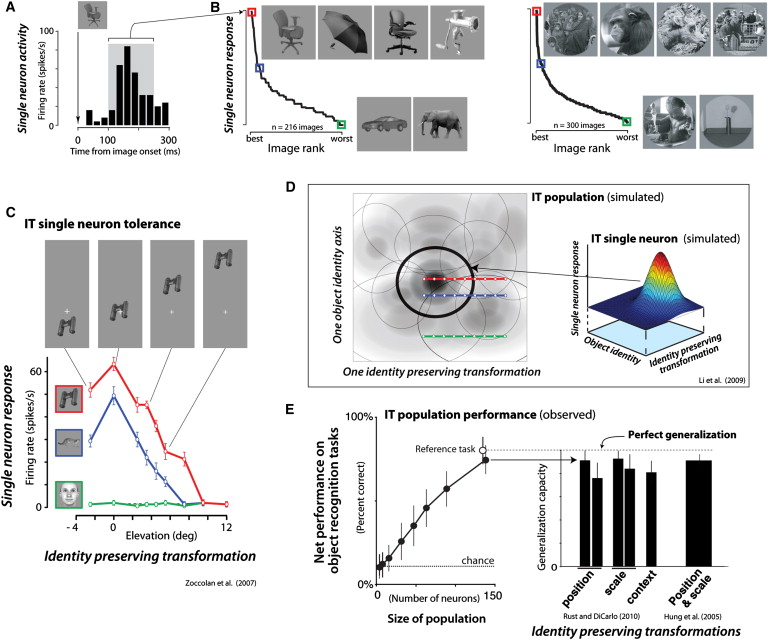
\includegraphics[width=0.9\textwidth]{pics_report/IT.jpg}
%	\caption{	
%		IT single-neuron properties and their relationship to population performance~\cite{dicarlo2012does}.
%	}
%	\label{Fig:IT}
%\end{figure}
%Most studies have investigated the neural activities in the IT by means of firing rate or spike count.
%A typical histogram, Figure~\ref{Fig:IT}(A)~\cite{zoccolan2007trade}, shows the spike count of a single neuron in time bins of 25~ms for a duration of 300~ms in total right after the presentation of a visual image.
%The highlighted time window, the so-called `decoding' window, is adjusted to the latency of the conductance along the ventral stream. 
%The spike count of the `decoding' window is well modulated for object identity, position or size~\cite{desimone1984stimulus,kaneko1996sequence}, see example in Figure~\ref{Fig:IT}(B) where the left shows the spiking activities for clean figures and the right for natural scenes.
%The neural responses were sorted from high to low with the corresponding figures presented, where the red point indicated the highest respond while the green the lowest and the blue the medium.
%Another example in Figure~\ref{Fig:IT}(C) shows the responses of an example IT neuron obtained by varying the position (elevation) of three objects with high (red), medium (blue), and low (green) activities.
%The object identity preference was maintained in the entire test range regardless of the position changes.
%These tuning curves are similar to the well-understood firing rate modulation in visual area V1 on the bar orientation.
%
%%A Contemporary View of IT Single Neurons\\
%%Respond to different variations\\
%%How do these IT neuronal population phenomena (above)
%%depend on the responses of individual IT neurons?
%Understanding IT single neuron responses has proven to be extremely challenging and even predicting the responses of an IT neuron to a new image remains impossible.
%Nevertheless, IT neurons are activated by complex combinations of visual features and that they are often able to maintain their relative object preference over small to moderate changes in object position, scale, pose~\cite{logothetis1996visual}, illumination~\cite{vogels2002effects} and clutter~\cite{zoccolan2005multiple}.
%
%%respond to more objects\\
%Although IT neurons are commonly described as narrowly selective object identifier, neurophysiological studies have shown a diverse selectivity of single neurons~\cite{desimone1984stimulus}.
%Most IT neurons are broadly tuned and the typical IT neuron responds to many different images and objects~\cite{zoccolan2007trade}, also see Figure~\ref{Fig:IT}(B).
%As illustrated in Figure~\ref{Fig:IT}(D), a single neuron (right) is modulated to both object identities and variables of identity-preserving transformations.
%To explain the plot in ~\ref{Fig:IT}(C), position is the variable here; thus the tuning curve for different identities on each position can be described as a slice in the 3-D plot which is Gaussian-like.
%As a result, the rank order of the three objects remains the same due to the Gaussian-like curve stays similar.
%If a population of such IT neurons tiles with the overlapping fashion, see left panel of Figure~\ref{Fig:IT}(D), a more accurate recognition result containing the transformation parameter can be carried out with population coding.
%
%\subsubsection{Population of neurons}
%
%Spike timing variability in the ms resolution of spikes is consistent with a Poisson-like stochastic spike generation process.
%The underlying output rate of IT neurons is determined by each particular image.
%Despite the timing variability, the brain can reliably recognise the presented object by integrating the neural responses across IT population~\cite{de2007properties}.
%However, it still remains unclear whether the spike timing variability brings down the encoding/decoding accuracy or if it contributes to the population tuning for useful informations~\cite{ermentrout2008reliability}. 
%
%%simple weighted summations of IT spike\\
%Although the first stage of the ventral stream, V1, is reasonably well studied, the visual processing in higher stages especially in V4 and IT remains poorly understood.
%Nevertheless, as stated above IT is the main part of ventral stream to recognise and categorise the objects in real-time and is tolerant to identity-preserving transformations.
%Specifically, simple linear classifier built on the output rates of randomly selected population with only a few hundred neurons reveals a high-level of object recognition performance~\cite{hung2005fast};
%and the simple weighted summation explains a wide range of invariant object recognition behaviour sufficiently~\cite{majaj2012unified}.
%
%Figure~\ref{Fig:IT}(E) shows the direct tests of measuring the cross-validated population performance on categorisation tasks using linear classifiers.
%The recognition performance approaches ceiling level with only a few hundred neurons (left panel), and the same population shows a good generalization across moderate changes in position, scale, and context.
%%50 ms window matters\\
%\subsubsection{Decoding Window Matters}
%The output spiking pattern of the ventral visual stream are well described by a firing rate code where the decoding window size is 50~ms~\cite{hung2005fast}.
%Thus the visual representation in IT is usually found in the first 50~ms of neuronal response, although different time epochs relative to stimulus onset may encode different types of visual information~\cite{brincat2006dynamic} (see Figure~\ref{Fig:IT}(A), an appropriate decoding window can be 100-150~ms after image onset).
%
%%\subsection{IT}
%
%
%
%
%%conclusion\\
%%Such findings argue for a distributed representation of visual
%%objects in IT, as suggested previously (e.g., Desimone et al.,
%%1984; Kiani et al., 2007; Rolls and Tovee, 1995)—a view that
%%motivates the population decoding approaches described
%%above (Hung et al., 2005; Li et al., 2009; Rust and DiCarlo,
%%2010). That is, single IT neurons do not appear to act as sparsely
%%active, invariant detectors of specific objects, but, rather, as
%%elements of a population that, as a whole, supports object recog-
%%nition. This implies that individual neurons do not need to be
%%invariant. Instead, the key single-unit property is called neuronal
%%‘‘tolerance’’: the ability of each IT neuron to maintain its prefer-
%%ences among objects, even if only over a limited transformation
%%range (e.g., position changes; see Figure 4C; Li et al., 2009).
%%Mathematically, tolerance amounts to separable single-unit
%%response surfaces for object shape and other object variables
%%such as position and size (Brincat and Connor, 2004; Ito et al.,
%%1995; Li et al., 2009; Tove ́e et al., 1994; see Figure 4D). This
%%contemporary view, that neuronal tolerance is the required and
%%observed single-unit phenomenology, has also been shown for
%%less intuitive identity-preserving transformations such as the
%%addition of clutter (Li et al., 2009; Zoccolan et al., 2005).
%
%
%%Summery\\
%%Taken together, the neurophysiological evidence can be
%%summarized as follows. First, spike counts in 50 ms IT decod-
%%ing windows convey information about visual object identity.
%%Second, this information is available in the IT population begin-
%%ning 100 ms after image presentation (see Figure 4A). Third,
%%the IT neuronal representation of a given object across changes
%%in position, scale, and presence of limited clutter is untangled
%%from the representations of other objects, and object identity can
%%be easily decoded using simple weighted summation codes (see
%%Figures 2B, 4D, and 4E). Fourth, these codes are readily
%%observed in passively viewing subjects, and for objects that
%%have not been explicitly trained (Hung et al., 2005). 
%
%In sum, the output of the ventral stream is reflexively expressed in neuronal firing rates across a short interval of 50 ms and is an explicit object representation;
%and the rapid production of this representation is consistent with a largely feed-forward, non-linear processing of the visual input~\cite{dicarlo2012does}, which is described in the following section.
%\subsection{Hierarchical Feed-forward Organisation }
%%Feed-forward, hierarchical organisation and abstraction.
%
%\begin{figure}[h!]
%	\centering
%	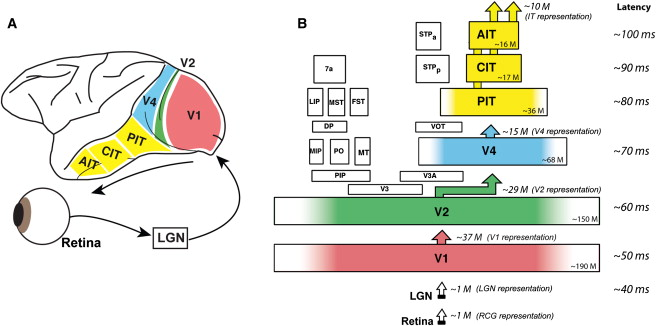
\includegraphics[width=0.9\textwidth]{pics_report/ventral.jpg}
%	\caption{The ventral visual pathway and its hierarchical organization~\cite{dicarlo2012does}.
%}
%	\label{Fig:Ventral}
%\end{figure}
%Figure~\ref{Fig:Ventral}(A) illustrates the ventral stream cortical area locations in the macaque monkey brain, and the flow of visual information from the retina.
%The corresponding hierarchical organisation is showed in Figure~\ref{Fig:Ventral}(B).
%Each area is plotted with the size proportional to its cortical surface size.
%Approximate total number of neurons of both hemispheres is shown in the corner of the cortical areas.
%The approximate number of projections is written above each block.
%In addition, the colour dedicates to processing the central 10$^\circ$ of the visual field.
%At last, approximate median response latency is listed on the right.
%%of the ventral stream with spikes travelling first from the retina to the lateral geniculate nucleus of the thalamus (LGN), and then through cortical areas introduced above: V1 , V2, V4 to IT. 
%\subsubsection{Latency}
%Each cortical area along the ventral stream contributes a conductance latency of about 10~ms of the visual information~\cite{nowak1997timing}.
%Thus, just around 100~ms after images appeared in front of the retina, a first wave of object identity neuronal activity is present throughout much of IT (e.g., Figure~\ref{Fig:IT}(A)).
%
%\subsubsection{Neurons and Connections}
%Because retinal and LGN receptive fields are point-wise spatial sensors, the object visual information conveyed to V1 are nearly as raw as the pixel representation (1 million pixels). 
%As V1 carries out its visual process, the total object representation increases approximately 30-times~\cite{stevens2001evolutionary} because of its non-linear filtering.
%This dimensionality expansion results in an overcomplete population re-representation~\cite{lewicki2000learning} in which the object representation vectors have more dimensions than the LGN input.
%As a result, simulations show that a V1-like representation is clearly better than RGN-like/pixel-based representation, but still far below human performance for real-world recognition problems~\cite{dicarlo2007untangling}.
%
%The output projections of each area decreases from V2 (about 29 million) to AIT which represents the object with 10 million dimensions.
%At the same time, the receptive field size of neurons increases to complete the object representation with a whole image and to perform invariant recognition.
%
%%\begin{figure}
%%	\centering
%%	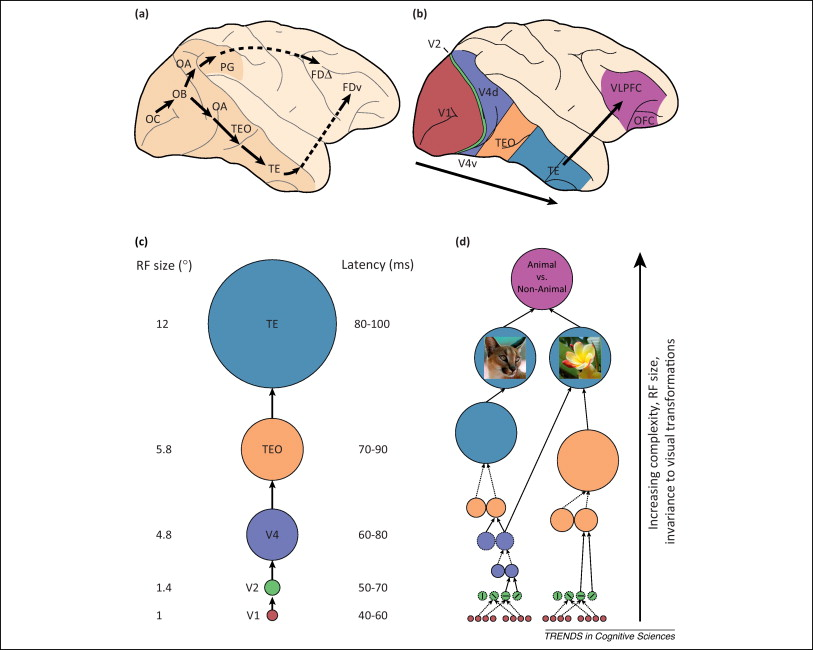
\includegraphics[width=0.9\textwidth]{pics_report/hierarchi.jpg}
%%	\caption{Receptive field sizes of the sub areas along the hierarchical visual processing pathway~\cite{kravitz2013ventral}.}
%%	\label{Fig:Hir1}
%%\end{figure}
%\subsubsection{Tuned Features and Receptive Fields }
%\begin{figure}[h!]
%	\centering
%	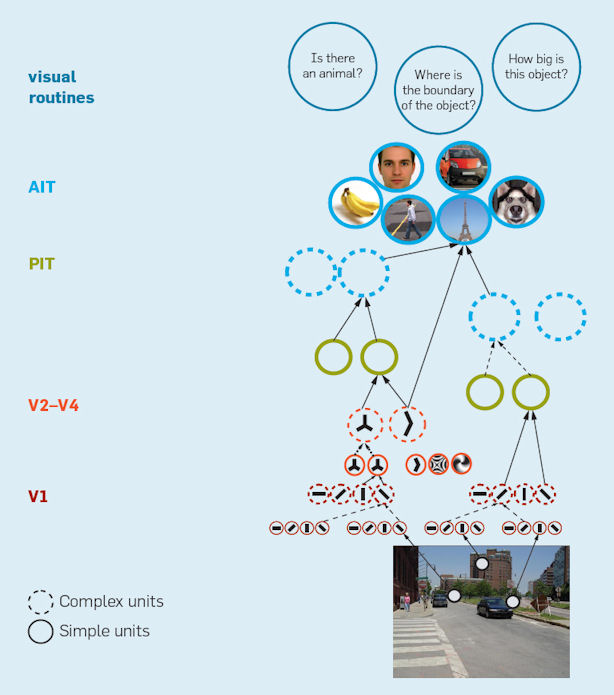
\includegraphics[width=0.9\textwidth]{pics_report/serre.jpg}
%	\caption{The hierarchical ventral stream and the corresponding tuned features for each layer~\cite{serre2010neuromorphic}.}
%	\label{Fig:serre}
%\end{figure}
%As the visual information conducts along the ventral stream, neurons become selective for stimuli that are increasingly complex from simple oriented bars and edges in early visual area V1 to moderately complex features in intermediate areas: V2, V4 and PIT to complex objects and faces in AIT, see Figure~\ref{Fig:serre}.
%Along with this growing complexity of the preferred stimulus, the invariance properties of neurons also increase.
%Neurons become more and more tolerant with respect to the exact position and scale of the stimulus within their receptive fields.
%As a result, the receptive field size of neurons increases from
%about one degree or less in V1 to several degrees in IT, see Figure~\ref{Fig:Hir1}.
%
%\begin{figure}[h!]
%	\centering
%	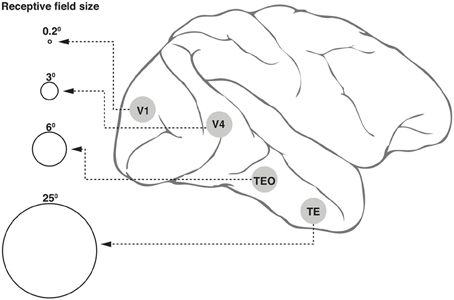
\includegraphics[width=0.6\textwidth]{pics_report/rf.jpg}
%	\caption{Receptive field (RF) sizes along the ventral cortical stream in the primate. While the degree of complexity of processing may increase, the RF size at any one eccentricity also increases dramatically along the various cortical areas from V1 into the temporal pole. The circles shown in the figure are not drawn to scale, but the numbers above the circles indicate approximate relative sizes of the RF diameters.~\cite{vidyasagar2013reading}.}
%	\label{Fig:Hir1}
%\end{figure}
%
%%\subsubsection{Tuned Features}
%%
%%V1 are orientation selective for multiple stimulus types, i.e., edges, bars, gratings (Hubel and Wiesel, 1968; Hubel et al., 1978).
%%V2 cells encode border ownership (Zhou et al., 2000) which is the first stage of assigning an oriented edge to an object representation.
%%Thus contour-based object representation starts in V2.
%%Form processing in V4 combines multiple, spatially-adjacent, orientation responses seen in V1 and V2 to encode angles and curvatures (Pasupathy and Connor, 1999).
%%These responses advance the nascent object representation from border ownership (Orban, 2008) to responses that are dependent on the placement of the curvature with respect to the center of the shape (Pasupathy and Connor, 2001).
%%
%%Inferior temporal (IT) cortex has a range of object property complexity starting with simpler features posteriorly (PIT or TEO: Tanaka et al., 1991; Kobatake and Tanaka, 1994) that increase in complexity as processing moves anteriorly (AIT or TE) to represent objects and perform object recognition (Cowey and Weiskrantz, 1967; Gross et al., 1971, 1972; Dean, 1976).
%%This includes complex shapes, combinations of color or texture with shape (Gross et al., 1972; Desimone et al., 1984; Tanaka et al., 1991), and body parts (faces or hands: see Gross, 2008 for a review). 
%%In addition, responses in IT cortex are position and size invariant (Sato et al., 1980; Schwartz et al., 1983; Rolls and Baylis, 1986; Ito et al., 1995; Logothetis and Pauls, 1995) and also invariant to changes in luminance, texture, and relative motion (Sáry et al., 1993).
%%Combined, these characteristics make IT ideal for representing objects despite changes in the surrounding environment and retinal image.
%
%%
%%\begin{figure}
%%	\centering
%%	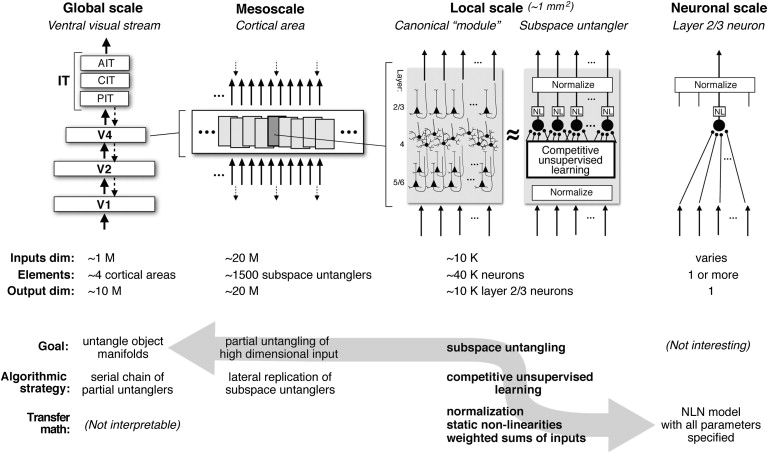
\includegraphics[width=0.9\textwidth]{pics_report/hierarchiNLN.jpg}
%%	\caption{The ventral visual pathway and its hierarchical organization~\cite{dicarlo2012does}.}
%%	\label{Fig:HirNLN}
%%\end{figure}

\section{Computational Neuroscience: what and why spiking neurons}
\label{sec:comp}

%\section{Spatial Temporal Learning}
%\label{sec:stl}
The so-called third generation of neural networks~\cite{maass1997networks} introduces a different set of functions and parameters to model neurons;
%these both model biological neurons more precisely~\cite{hodgkin1952quantitative} and increase the computational power of networks of neurons if compared to classical sigmoidal units.
it models the biological neurons more precisely and increases the computational power of neural networks when compared to the classical sigmoid functions.
Such networks rely on the propagation of an all-or-none signal, the action potential, which asynchronously carries information to its connected units by means of its timing.
\subsection{Neuronal Model}
Spiking neuron models can be divided into two major categories \cite{gernstbook} based on their level of abstraction: The conductance models and the threshold models.
The conductance models simulate a lower level on the ion channels, while the threshold models represent a higher level of neuron abstraction where the threshold voltage is fixed and the neuron fires once the membrane potential reaches it.

In general, Conductance-Based models have been derived from the Nobel prize winners (1963) Hodgkin and Huxley, based on the experiments that they performed on the giant axon squid \cite{hhmodel}.
Spikes arriving at a LIF neuron cause a temporary flow of current into (excitatory synapse) or out of (inhibitory synapse) the neuron, modelling the behaviour of synapses in biological neurons.
The LIF neuron sums up this current over time, accumulating charge which gradually leaks away.
If the membrane potential in the neuron reaches a certain threshold, it produces a spike and its charge is reset.
LIF neurons have been extensively used in large spiking neural networks \cite{Delorme1999989} because of their ease of implementation and the low computational cost.

\subsection{Learning}
%One of the key parameters of a neural network is the amount of influence each incoming spike has on a neuron.
The influence each incoming spike has on a post-synaptic neuron is modelled by assigning a `weight' to each synapse;
tuning on the weight scales the impact of a spike
arriving via that synapse.
Many learning models simulate the changes in weights over long periods of time observed within the brain.
The exact rules by which these weights are adjusted is the subject of much active research though most promising approaches attempt to learn from the relative timing \cite{pfister2006triplets} or rate \cite{bienenstock1982theory} of spikes arriving at a neuron.
As well as adjusting weights, some learning rules can also form entirely new connections between previously unconnected
neurons \cite{bamford2010synaptic}.

\section{Neuromorphic Engineering}
\label{sec:morph}

\section{Deep Learning}
\subsection{Convolutional Network}
\subsection{Autoencoders}
\label{sec:AE}
Figure~\ref{fig:AE} shows a simplest architecture of an autoencoder, which is the same as a multilayer perceptron (MLP).
The only difference lies to the number of the output units, where an autoencoder has as many output neurons as the input.
In this example, the input layer feeds forward the data vector $\mathbf{v}$ to the hidden layer as weighted sum of the data, $\mathbf{net\_h}$.
Then the hidden units are activated by the input $\mathbf{net\_h}$ according to the activation function: $\mathbf{h}=\sigma(\mathbf{net\_h})$.
Finally, using the same approach the output of the network is generated, $\mathbf{v'}=\sigma(\mathbf{net\_v'})$, as the reconstruction of the input data.
Thus, autoencoders are trained without given target values, work as unsupervised learning models.
\begin{equation}
h_j=\sigma(\sum_i v_i w^T_{ij})
\end{equation}
\begin{equation}
v'_j=\sigma(\sum_i h_i w_{ij})
\end{equation}

\begin{figure}
	\centering
	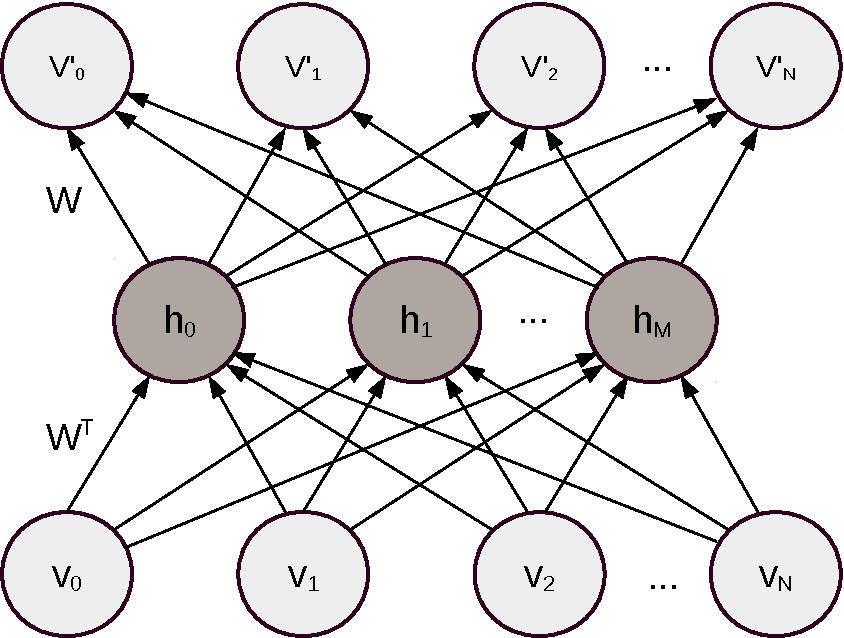
\includegraphics[width=0.5\textwidth]{pics_sdlm/AE.pdf}
	\caption{A typical Autoencoder structure.}
	\label{fig:AE}
\end{figure}

%TODO why tied weights are good
Notice that the connections used in the example are tied weights.

Training an autoencoder is not different from backpropagation (BP) on an Multi-Layer Perceptrons(MLP).
The objective of training is to minimise the prediction error of an MLP, which measured as a loss function.
Accordingly, the loss function of an autoencoder can be described as:
\begin{equation}
L=\sum_{k=1}^{K}\|\mathbf{v}_{k}-\mathbf{v'}_{k}\|=\frac{1}{2}\sum_{k=1}^{K}(\mathbf{v}_{k}-\mathbf{v'}_{k})^{2}
\end{equation}
where k indicates the index of the training data $\mathbf{v}$, and each data vector $\mathbf{v}=\{v_0, v_1,...,v_N\}$ and its reconstruction $\mathbf{v'}=\{v'_0, v'_1,...,v'_N\}$ have N dimensions. 

%TODO rewording
Backpropagation, an abbreviation for "backward propagation of errors", is a common method of training artificial neural networks used in conjunction with an optimization method such as gradient descent.
The method calculates the gradient of a loss function with respect to all the weights in the network.
The gradient is fed to the optimisation method which in turn uses it to update the weights, in an attempt to minimise the loss function:
\begin{equation}
\Delta W \propto -\frac{\partial L}{\partial W}.
\end{equation}

Applying stochastic gradient descent (SGD), the true gradient of the weight matrix, $\Delta W$, is approximated by a gradient at a single example with iterations.
The reconstruction error $E_k$ of an input vector $\mathbf{v}_k$ is as given:
\begin{equation}
%	\begin{align*}
E_k = \frac{1}{2}(\mathbf{v}_k - \mathbf{v'}_k)^2,
%	\end{align*}
\end{equation}
and the gradient of the weight matrix is:
\begin{equation}
\Delta W \propto -\frac{\partial E_k}{\partial W}=-\eta \frac{\partial E_k}{\partial W},
\end{equation}
where $\eta$ is the learning rate.

Since we use tied weights in the network, the weight tuning only needs to apply in the output layer.
\begin{equation}
\begin{aligned}
\Delta w_{ij} = -\eta \frac{\partial E_k}{\partial w_{ij}} &= -\eta \frac{\partial E_k}{\partial v'_j} \frac{\partial v'_j}{\partial net\_v'_j} \frac{\partial net\_v'_j}{\partial w_{ij}}, \textrm{ where} \\
\frac{\partial E_k}{\partial v'_j} &= \frac{\partial \frac{1}{2} \sum_l (v_l - {v'}_l)^2}{\partial v'_j}= \frac{\partial \frac{1}{2}(v_j - {v'}_j)^2}{\partial v'_j}= v'_j - v_j, \\
%	\frac{\partial v'_j}{\partial net\_v'_j} &= \begin{cases} 1, v'_j>0\\0, v'_j<=0\\ \end{cases}, \textrm{using ReLU,}\\
\frac{\partial v'_j}{\partial net\_v'_j} &=\left\{
	\begin{aligned}
    & 1, net\_v'_j > 0 \\
    & 0, net\_v'_j < = 0
    \end{aligned} 
    \right.    \textrm{using ReLU, }\\
\frac{\partial net\_v'_j}{\partial w_{ij}} &= \frac{\partial h_i w_{ij}}{\partial w_{ij}} = h_i.
\end{aligned}
\end{equation}
Thus, the weight gradient is calculated as:
\begin{equation}
\label{equ:ae_widrow_hoff}
\Delta w_{ij} = \left \{
	\begin{aligned}
	& \eta h_i(v_j - v'_j), &net\_v'_j > 0 \\
	&-\eta h_i v'_j, & net\_v'_j < = 0
	\end{aligned} 
	= \eta h_i(v_j - v'_j)
\right.
\end{equation}

\subsection{Restricted Boltzmann Machine}
\label{sec:rbm}
In order to implement training and testing of Spiking Deep~Belief~Networks~(SDBNs) on-line, this section studied:
\begin{itemize}
	\item \textit{Contrastive Divergence.}
	The study starts from understanding the original problem, Products of Experts~(PoE), which was solved by using Contrastive~Divergence~(CD).
	It involves utilising Markov~Chain~Monte~Carlo~(MCMC) sampling to present the distribution of a certain untraceable high-dimensional probability model function, e.g. PoE.
	Among these sampling algorithms, Gibbs method is introduced and used in high dimensional problems.
	Instead of minimising the original objective function of Kullback-Leibler divergence, the contrastive divergence is exploited to solve PoE.
	\item \textit{Restricted Boltzmann Machine (RBM). }
	Then the study continues on applying Gibbs sampling and CD to RBM, which builds the foundation of the light RBM training.
	\item \textit{Deep Belief Network.} 
	The greedy algorithm on training layered RBMs and the fine training on the whole DBN are studied.
\end{itemize}
Next, the study will carry on to on-line learning methods which only applies to spiking neurons for training spiking RBM and DBN.
\subsubsection{Contrastive Divergence\cite{hinton2002training,woodfordnotes}}
The probability of a vector point $ \mathbf{x} $ is modelled by the function $f(\mathbf{x} \mid \Theta )$ given the model parameters $ \Theta $, and normalised by a partition function $Z( \Theta)$:

\begin{equation}
p(\mathbf{x} \mid \Theta ) = \dfrac{f(\mathbf{x} \mid \Theta )}{Z( \Theta)}
\end{equation}
where the partition function is defined as:
\begin{equation}
\label{equ:z_int}
Z( \Theta) = \int f(\mathbf{x} \mid \Theta )\D\mathbf{x}, \text{when  $ \mathbf{x} $ is continuous, or}
\end{equation}

\begin{equation}
\label{equ:z_dis}
Z( \Theta) = \sum_{\mathbf{x}} f(\mathbf{x} \mid \Theta ), \text{when  $ \mathbf{x} $ is discrete.}
\end{equation}
Given a set of data points $ \mathbf{D}=(\mathbf{d}_1, \mathbf{d}_2, ..., \mathbf{d}_K) $ the purpose of learning is to tune the model parameter $ \Theta $ to fit the data $ \mathbf{D}  $. 
The objective function is the probability product of all the independent data points of the data set, which is also called the likelihood function:
\begin{equation}
L (\Theta \mid \mathbf{D}) = p(\mathbf{D} \mid \Theta ) = \prod_{k=1}^K p(\mathbf{d}_k \mid \Theta ) =  \prod_{k=1}^K\dfrac{f(\mathbf{d}_k \mid \Theta )}{Z( \Theta)}.
\end{equation}
And the target is to maximise the likelihood given the data set $ \mathbf{D}  $, which equals to maximise the log of the probability product (the log-likelihood):
\begin{equation}
\log  L (\Theta \mid \mathbf{D}) = \log p(\mathbf{D} \mid \Theta ) = \sum_{k=1}^K\log f(\mathbf{d}_k \mid \Theta ) - K \log Z( \Theta),
\end{equation}
or the average log-likelihood:
\begin{equation}
\label{equ:like}
\hat{l} (\Theta \mid \mathbf{D}) =\frac{1}{K}\log  L (\Theta \mid \mathbf{D}) 
=\frac{1}{K}\sum_{k=1}^K\log f(\mathbf{d}_k \mid \Theta ) - \log Z( \Theta).
\end{equation}
Imagine three different conditions (probability function) as following.

\textbf{First}, $f(\mathbf{x} \mid \Theta )$ is the probability density function (pdf) of a normal distribution $\mathcal{N}(x \mid \mu, \sigma )$.
Data vector $ \mathbf{x} $ is just a one dimensional data point, $x$.
$ Z( \Theta) $ equals to 1, thus $p(x \mid \Theta ) = \mathcal{N}(x \mid \mu, \sigma )$.
\begin{equation}
\hat{l} (\Theta \mid D) =  
\frac{1}{K} \sum_{k=1}^K \log \left[ \frac{1}{\sigma \sqrt{2\pi}} \exp(-\frac{(d_k-\mu)^{2}}{2\sigma^{2}}) \right]
\label{pdf}
\end{equation}
To maximise Equation~\ref{pdf} is to find the Maximum Likelihood Estimation (MLE) of parameters $ \mu $ and $ \sigma $, by deriving from the partial differential equations when they are equal to 0. 
\begin{equation}
\left\{
\begin{aligned}
&\dfrac{\partial \hat{l} (\Theta \mid D)}{\partial \mu}= \sum_{k=1}^K -\frac{1}{2\sigma^{2}}\dfrac{\partial (\mu-d_k)^{2}}{\partial \mu} = \sum_{k=1}^K -\frac{1}{\sigma^{2}}(\mu-d_k) = 0 \quad\\
&\dfrac{\partial \hat{l} (\Theta \mid D) }{\partial \sigma^{2}}= -\frac{K}{2\sigma^{2}}+\frac{1}{2\sigma^{4}}\sum_{k=1}^K d_k^{2} -\frac{\mu}{\sigma^{4}}\sum_{k=1}^K d_k + \frac{K\mu^{2}}{2\sigma^{4}} = 0 \quad\\
\end{aligned}
\right.
\end{equation}
\begin{equation}
\left\{
\begin{aligned}
&\mu= \frac{1}{K}\sum_{k=1}^K d_k  \quad\\
&\sigma^{2} = \frac{1}{K}\sum_{k=1}^K d_k^{2} - (\frac{1}{K}\sum_{k=1}^K d_k)^{2}
\end{aligned}
\right.
\end{equation}
$\hat{l} (\Theta \mid D)$ here is the function of two dimensional parameters $\mu$ and $\theta$, and searching the highest point in the parameter space ``is equivalent to being in the field on a clear, sunny day,''~\cite{woodfordnotes} seeing the point straight away.

\textbf{Second}, the probability model function changes to be the sum of N normal distributions: 
\begin{equation}
f(x \mid \Theta ) = \sum_{i=1}^N\mathcal{N}(x \mid \mu_i, \sigma_i ).
\end{equation}
Derived from Equation~(\ref{equ:like}), the objective function is:
\begin{equation}
\hat{l} (\Theta \mid D) = \frac{1}{K}\sum_{k=1}^K \log \sum_{i=1}^N \mathcal{N}(d_k \mid \mu_i, \sigma_i ) - \log N,
\end{equation}
where $\log Z( \Theta)$ still equals a constant, but the partial differential equation of any parameter depends on other model parameters.
It is very hard to solve equation set of log of sum, thus iteration methods are introduced, e.g., gradient descent method. %and expectation maximization (EM) algorithm
Searching for a local maximum of the likelihood function in the parameter space starts with an initial point, either random or well selected.
For each iteration, the partial derivatives for every dimension of the parameter point are calculated as the gradient.
The gradient determines the decent direction of the space search, the next parameter point is one step $ \eta $  towards the direction or is the highest point found by line search.

The gradient descent method is equivalent to ``being in the field at night with a torch.''~\cite{woodfordnotes}.
And then the descent direction is estimated and chosen by using the torch to see the relative heights of the field a short distance in each direction.
Because partial differential equation of any parameter depends on other model parameters, we can only see the gradient for a small area.
The search will follow the direction by walking one step or a certain distance (e.g. line search lowest point), and then start a new iteration.

\paragraph{PoE Problem} 
%\subsubsubsection{PoE Problem}
\textbf{Finally}, the probability model function becomes the product of N normal distributions: 
\begin{equation}
f(x \mid \Theta ) = \prod_{i=1}^N\mathcal{N}(x \mid \mu_i, \sigma_i ),
\end{equation}
where the partition (normalisation) function $Z( \Theta)$ is no longer a constant, but varies accordance to all the parameters.
Essentially, the integration of the probability model, see Equation~(\ref{equ:z_int}) and~(\ref{equ:z_dis}), is usually algebraically intractable.
We have to use numerical integration method to evaluate the Equation~(\ref{equ:like}), whose partial derivative is (we are using vectors to generalise the problem):
\begin{equation}
\label{equ:part}
\begin{aligned}
\dfrac{\partial \hat{l} (\Theta \mid \mathbf{D})}{\partial \theta} 
& = \frac{1}{K} \dfrac{\partial \sum_{k=1}^K\log f(\mathbf{d}_k \mid \Theta )}{\partial \theta} - \dfrac{\partial \log Z( \Theta)}{\partial \theta}\\
& =  \frac{1}{K}\sum_{k=1}^K \dfrac{\partial \log f(\mathbf{d}_k \mid \Theta)}{\partial \theta} - \int p(\mathbf{x} \mid \Theta) \dfrac{\partial \log f(\mathbf{x} \mid \Theta)}{\partial \theta} \D \mathbf{x}\\
& = \left \langle \dfrac{\partial \log f(\mathbf{d} \mid \Theta)}{\partial \theta}\right \rangle_{\mathbf{D}} -\left \langle \dfrac{\partial \log f(\mathbf{c} \mid \Theta)}{\partial \theta}\right \rangle_{\mathbf{C} \sim p(\mathbf{x} \mid \Theta)}  \\
&=\left \langle \dfrac{\partial \log f(\mathbf{x} \mid \Theta)}{\partial \theta}\right \rangle_{\mathbf{X}_{data}} - \left \langle \dfrac{\partial \log f(\mathbf{x} \mid \Theta)}{\partial \theta}\right \rangle_{\mathbf{X}_{model}},
\end{aligned}
\end{equation}
where  $ <\cdot>_x $ denotes the mean expectation of $ \cdot $ given distribution of $x$.
The first term of the right-hand side is easy to get with the given data set $ \mathbf{D} $, and the second term can be approximated by generating data samples $ \mathbf{C} $ according to $ p(\mathbf{x} \mid \Theta) $.
These generative samples is called ``fantasy data'' and can be generated using Monte Carlo Markov Chain (MCMC) sampling, see section~\ref{sec:mcmc}.
The detailed derivation process can be found in Appendix~\ref{app:part}.
Although in this example the integration of product of normal distribution is still tractable, it is also helpful to use numerical integration.

Go back to the metaphor of the parameter field, solving PoE problem is like searching the highest point in a completely dark night without a torch.
The computation of Equation~(\ref{equ:part}) is to ``feel the gradient of the field under our feet''.~\cite{woodfordnotes}.
%The motivation underlining Contrastive Divergence algorithm is to boost the training speed of a Markov Chain in order to represent the distribution of a PoE (Product of Expert) model.
%Thus the sampling can be followed using this trained Markov Chain model. 

\paragraph{MCMC Sampling}
%\subsubsubsection{MCMC Sampling}
\label{sec:mcmc}
In order to solve the integration of algebraically intractable equations we can use numerical integration to approximate.
One of the popular method is Monte Carlo integration:
\begin{equation}
\int_{a}^{b} f(x) \D x = \int_{a}^{b}\frac{f(x)}{q(x)}q(x)\D x = \dfrac{1}{N}\sum_{i=1}^{N}\frac{f(x_i)}{q(x_i)}.
\end{equation}
The integration of $ f(x) $ transforms to the integration of a new function $ F(x) = f(x)/q(x)  $ times its probability function $ q(x) $.
It could be approximated by sampling N data points $ x_i $ according to the probability distribution $ q(x) $, and calculate the average of $ F(x_i) $ as $ <F(x)>_{q(x)}$.
So the main question following is how to sample from a probability distribution.

MCMC algorithm was proposed by Metropolis in 1953 and it became a wide-used sampling method.
The stationary distribution $ \pi $ exists when every two nodes in a Markov Chain are connected regardless of the initial state distribution $ \pi_0 $:
\begin{equation}
\begin{aligned}
&\pi(j) = \sum_{i=1}^{\infty}\pi(i)P_{ij} \\
&\pi P = \pi,
\end{aligned}
\end{equation}
where $ P $ is the transition probability matrix, and $ \pi $ is in the state space of a MC and the sum, $ \sum_{i=1}^{\infty}\pi(i) $,of a state distribution is 1.
Thus based on the useful theorem of MC, sampled sequence $ \{x_0, x_1, ..., x_n, ... \}$ from a MC complies with its stationary distribution $ \pi(x) $.
Metropolis stated that if a MC has a stationary distribution, $ q(x) $, which is exactly needed to sample from, then we can easily obtain a sample sequence along the MC according to the transformation probability matrix $ P $.
Here so far we are describing the MC with discrete states, however the it also applies to continuous $ \pi $ and $ P $.
The problem here is to build $ P $ to make the stationary distribution equal to the required probability, $ \pi(x) = q(x) $.

So the other useful theorem (detailed balance) lies here, if an aperiodic MC is reversible: $\pi (i) P_{ij} = \pi (j) P_{ji},$ then $ \pi $ is the stationary distribution.
It is a stronger condition than the previous theorem, so most of the MCs are not generally eligible:
\begin{equation}
\pi (i) P_{ij} \neq \pi (j) P_{ji}.
\end{equation}
Thus we can introduce another parameter matrix, $ \alpha $ to make a general MC reversible:
\begin{equation}
\pi (i) P_{ij} \alpha_{ij} = \pi (j) P_{ji} \alpha_{ji}	,
\end{equation}
where $ \alpha_{ij} = \pi(j) P_{ji} $ and $ \alpha_{ji} = \pi(i) P_{ij}$.
The altered transformation probability matrix is $ P'_{ij} =  P_{ij} \alpha_{ij}$ and $ P'_{ji} =  P_{ji} \alpha_{ji}$, and the MC complies the detailed balance condition: $\pi (i) P'_{ij} = \pi (j) P'_{ji}$.
The matrix parameter $ \alpha $ is called as ``acceptance rate'', and its physic meaning is as follows: when state $ i $ transforms to state $ j $ with a probability of $ P_{ij} $, the transformation is accepted by the rate of $ \alpha_{ij} $.
Since the accept rate may be too low for the sampling to move along the MC, we can normalise the $ \alpha $ pair to 1:
\begin{equation}
\alpha^{'}(i,j) = min \left\{\frac{\pi(j)P_{ji}}{\pi(i)P_{ij}},1\right\}.
\end{equation}
The algorithm is called Metropolis-Hastings and described in following:
\begin{algorithm}[h]
	\caption{Metropolis-Hastings Sampling}
	\label{alg:mcmc}
	\begin{algorithmic}
		
		%	    \Procedure{Correction}{coeffs $C$, correlations $Q$}
		\State Initialisation $x_0 = s_{random}$, \Comment{$ x $:sampling sequence and $s$:state in MC}
		\For{$t=1, 2, ..., N$}
		\State $y \sim p_(x \mid x_{t-1})$ 
		\Comment{Random drawing the next state by the transformation probability matrix $P$}
		\State $ u \sim Uniform[0,1] $ 
		\Comment{Random drawing from a uniform distribution}
		\If {$ u < \alpha^{'}(x_{t-1},y) = min \left\{\frac{q(y)p_(x_{t-1} \mid y)}{q(x_{t-1})p_(y \mid x_{t-1})},1\right\} $}
		\State {$x_t = y$} \Comment{Accept the transformation when the random number is less than $\alpha$}
		\Else \State {$x_t = x_{t-1}$}  \Comment{Transformation is refused elsewise}
		\EndIf
		\EndFor
	\end{algorithmic}
\end{algorithm}

The probability model function as the product of N normal distributions can be approximated by using this Metropolis-Hastings sampling.

\paragraph{Gibbs Sampling}
%\subsubsubsection{Gibbs Sampling}
\label{sec:Gibbs}
For high dimensional data sampling, it is possible to make the accept rate to 1 which increases the convergence speed dramatically.
According to conditional probability:
\begin{equation}
P(A \mid B) = \frac{P(A \cap B)}{P(B)}.
\end{equation}
For a $ n $ dimensional data $ (\mathbf{x}, y) $ where $ \mathbf{x}=(x_1,x_2,...,x_{n-1}) $, the joint probability of $p(\mathbf{x},y)$ is:
\begin{equation}
p(\mathbf{x},y) = p(y \mid \mathbf{x})p(\mathbf{x}).
\end{equation}
Thus, during sampling if we restrict the direction of transformation to one single axis(dimension), $ y $, from point $ A(\mathbf{x}_1, y_1) $ to point $ B(\mathbf{x}_1, y_2)$:
\begin{equation}
p(\mathbf{x}_1, y_1)p(y_2 \mid \mathbf{x}_1) = p(\mathbf{x}_1, y_2)p(y_1 \mid \mathbf{x}_1) = p(\mathbf{x}_1)p(y_1 \mid \mathbf{x}_1)p(y_2 \mid \mathbf{x}_1),
\end{equation}
then, the MC obeys the condition of detailed balance.
So the stationary distribution $ \pi(x_1,x_2,...,x_n) $ equals to the joint probability $ p(x_1,x_2,...,x_n) $ and the transformation probability matrix P is consisted of the conditional probability of each dimension $ k $ $,  p(x_k \mid x_1,...,x_{k-1},x_{k+1},...,x_n) $.
Therefore, given the conditional distribution of each variable for a multivariate distribution Gibbs sampling is able to approximate the joint distribution with long enough sample sequence.
Gibbs sampling is described as follows:
\begin{algorithm}[h]
	\caption{Gibbs Sampling}
	\label{alg:gibbs}
	\begin{algorithmic}
		
		%	    \Procedure{Correction}{coeffs $C$, correlations $Q$}
		\State Initialisation $\mathbf{x}_0 = [x_0(1),x_0(2),...,x_0(M)]$,  \Comment{Random initialise $\mathbf{x}_0$}
		\For{$t=1, 2, ..., N$}
		\For{$k=1, 2, ..., M$}
		\State $ x_t(k) = p(x(k) \mid x_{t-1}(1),x_{t-1}(2),...,x_{t-1}(k-1),x_{t-1}(k+1),...,x_{t-1}(M))$\\
		\Comment{Sampling by the conditional distribution}
		\EndFor
		\EndFor
	\end{algorithmic}
\end{algorithm}

\paragraph{CD Instead of KL(Kullback-Leibler)}
%\subsubsubsection{CD Instead of KL(Kullback-Leibler)}
\label{sec:CD}
Kullback-Leibler divergence is the measure of how different two probability distributions are:
\begin{equation}
\begin{aligned}
KL(P \mid \mid Q)
&= \int P(\mathbf{x}) \log \frac{P(\mathbf{x})}{Q(\mathbf{x})} \D \mathbf{x}\\
%= \sum_{\mathbf{x}} P(\mathbf{x}) \log \frac{P(\mathbf{x})}{Q(\mathbf{x})} \\
&= \int P(\mathbf{x}) \log P(\mathbf{x}) \D \mathbf{x} - \int P(\mathbf{x}) \log Q(\mathbf{x}) \D \mathbf{x}\\
%=  \sum_{\mathbf{x}} P(\mathbf{x}) \log P(\mathbf{x}) - \sum_{\mathbf{x}} P(\mathbf{x}) \log Q(\mathbf{x})\\
&= \left \langle \log P(\mathbf{x}) \right \rangle_{\mathbf{X} \sim P(\mathbf{x})} - \left \langle \log Q(\mathbf{x}) \right \rangle_{\mathbf{X} \sim P(\mathbf{x})} ,
\end{aligned}
\end{equation}
and the second term of the right hand side is the average log-likelihood function (see Equation~\ref{equ:like}) if $P(\mathbf{x})$ is the training data distribution and $Q(\mathbf{x})$ is the model distribution:
\begin{equation}
\begin{aligned}
& KL \left( p(\mathbf{x} \mid \mathbf{D}) \mid \mid p(\mathbf{x} \mid \Theta) \right)
=   \left \langle \log p(\mathbf{d} \mid \mathbf{D}) \right \rangle_{\mathbf{D}} - \left \langle \log p(\mathbf{d} \mid \Theta) \right \rangle_{\mathbf{D}}, \textit{where} \\
& \hat{l} (\Theta \mid \mathbf{D}) =\frac{1}{K}\log  L (\Theta \mid \mathbf{D}) 
=  \frac{1}{K}\log p(\mathbf{D} \mid \Theta ) 
= \frac{1}{K} \sum_{k=1}^{\mathbf{K}} \log f(\mathbf{d}_k \mid \Theta )
= \left \langle \log p(\mathbf{d} \mid \Theta) \right \rangle_{\mathbf{D}}.
\end{aligned}
\end{equation}
We use $ \mathbf{D} $ instead of $ \mathbf{X} \sim p(\mathbf{x} \mid \mathbf{D}) $, for $ p(\mathbf{x} \mid \mathbf{D}) $ is the distribution of data set $ \mathbf{D} $.
If we need to generate a sample sequence according to the distribution $ p(\mathbf{x} \mid \mathbf{D}) $, $ \mathbf{D} $ itself is the most approximated.
Since $\left \langle \log p(\mathbf{d} \mid \mathbf{D}) \right \rangle_{\mathbf{D}}$ is independent with model parameters, the negative partial derivative is the same with Equation~(\ref{equ:part}):
\begin{equation}
\label{equ:kl}
-\dfrac{\partial KL \left( p(\mathbf{x} \mid \mathbf{D}) \mid \mid p(\mathbf{x} \mid \Theta) \right)}{\partial \theta}
= \dfrac{\partial \hat{l} (\Theta \mid \mathbf{D})}{\partial \theta} \\
= \left \langle \dfrac{\partial \log f(\mathbf{d} \mid \Theta)}{\partial \theta}\right \rangle_{\mathbf{D}} - \left \langle \dfrac{\partial \log f(\mathbf{c} \mid \Theta)}{\partial \theta}\right \rangle_{\mathbf{C} \sim p(\mathbf{x} \mid \Theta)} .
\end{equation}
Therefore, for each iteration searching in the parameter space we use $ k $ number of training data $ \mathbf{D}=(\mathbf{d}_1, \mathbf{d}_2, ..., \mathbf{d}_k) $ and fantasy data $ \mathbf{C}=(\mathbf{c}_1, \mathbf{c}_2, ..., \mathbf{c}_k) $.
If $ k $ is big enough, sampling sequences $ \mathbf{D} $ and $ \mathbf{C} $ are able to approximate the data and the model distribution thus to get derivatives of the KL function.
However, if we just take a small number of data, even $ k = 1 $ per iteration~\cite{hinton2002training}, the KL divergence can be seen as a ``k-step contrastive convergence ($ CD_{k}) $'':
\begin{equation}
\label{equ:cdk}
\dfrac{\partial CD_{k}}{\partial \theta} 
= - \left \langle \dfrac{\partial \log f(\mathbf{d} \mid \Theta)}{\partial \theta}\right \rangle_{(\mathbf{d}_1, \mathbf{d}_2, ..., \mathbf{d}_k) } + \left \langle \dfrac{\partial \log f(\mathbf{c} \mid \Theta)}{\partial \theta}\right \rangle_{(\mathbf{c}_1, \mathbf{c}_2, ..., \mathbf{c}_k) \sim p(\mathbf{x} \mid \Theta)}.
\end{equation}
Since the searching step $ \eta $ is very small, the derivatives of points in a small area can be seen as the same.
%	The step made for a single $ CD_{k} $ can be approximated by summation of $ k $ steps of $ CD_{1} $ as long as the searching does not go far.
%	Otherwise the searching path may follow some direction for accumulated steps away from the original area, thus significantly reduces the training time.

\paragraph{Discussion}
%\subsubsubsection{Discussion}
Although there is practical explanation on using $CD_1$ for parameter space searching, arguments exist over whether the search converge to the same maxima/minima as $CD_\infty$~\cite{wu2015bias}.
Moreover, is the parameter searching still following the original objective function?	
As an initial exploration over the problem we tested some experiments on Section~\ref{sec:cd1}. 
%	Thus,
%	\begin{equation}
%		\dfrac{\partial [KL(p^0 \mid \mid p^{\infty}) - KL(p^1 \mid \mid p^{\infty})]}{\partial \theta}
%		= \left \langle \dfrac{\partial \log f(\mathbf{x} \mid \Theta)}{\partial \theta}\right \rangle_{\mathbf{p}^1} - \left \langle \dfrac{\partial \log f(\mathbf{x} \mid \Theta)}{\partial \theta}\right \rangle_{\mathbf{p}^0},
%	\end{equation}
%	where the second term in equation~(\ref{equ:kl}) cancels out.
%	So Hinton proposed \textcolor{red}{the new contrastive divergence CD to make Gibbs sampling with only 1 step}.
%	Contrastive divergence is defined as:
%	\begin{equation}
%		CD_n = KL(p^0 \mid \mid p^{\infty}) - KL(p^n \mid \mid p^{\infty})
%	\end{equation}
\subsubsection{RBM\cite{zhang2013rbm}}
RBM is a restricted version of Boltzman machine, where there are only connections between layers of units but not between units within a layer, see Figure~\ref{fig:RBM}.
$ v $ is the layer of visible units representing the observable data $ \mathbf{v} $, while $ h $ are the hidden units which can be seen as feature extractors.
The connections between the hidden layer and the visible layers are bidirectional weights, $ \mathbf{W} $.
Note that, both visible and hidden units have their bias individually, $ \mathbf{a} $ and $ \mathbf{b} $.
Thus the RBM consists of the data $ \mathbf{D} = \mathbf{V} = (\mathbf{v}_1, \mathbf{v}_2, ..., \mathbf{v}_K ) $, the model parameters $ \Theta = (\mathbf{a}, \mathbf{b}, \mathbf{W}) $ and the hidden units $ \mathbf{h} \sim p(\mathbf{h} \mid \mathbf{v}, \Theta) $.
\begin{figure}[hbt]
	\centering
	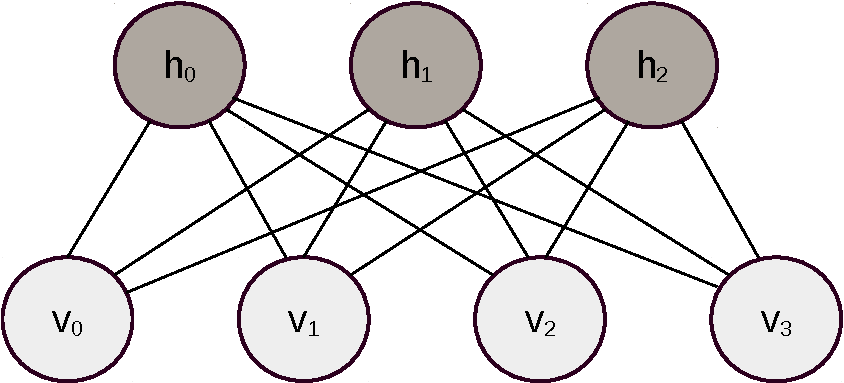
\includegraphics[width=0.6\textwidth]{pics_sdbn/RBM.pdf}
	\caption{A typical RBM structure.}
	\label{fig:RBM}
\end{figure}

The Energy function~\cite{hopfield1982neural} of a RBM is defined as follows, which has $ n $ vision units and $ m $ hidden ones:
\begin{equation}
E(\mathbf{v}, \mathbf{h} \mid \Theta)= -\sum_{i=1}^n a_i v_i - \sum_{j=1}^m b_j h_j - \sum_{i=1}^n \sum_{j=m}^n v_i W_{ij} h_j.
\end{equation}
And the model function and its probability functions are as follows:
\begin{equation}
\begin{aligned}
& f(\mathbf{v}, \mathbf{h} \mid \Theta) =e^{-E(\mathbf{v}, \mathbf{h} \mid \Theta)} \\
& p(\mathbf{v}, \mathbf{h} \mid \Theta) =\frac{e^{-E(\mathbf{v}, \mathbf{h} \mid \Theta)}}{Z(\Theta)}\\
& Z(\Theta) = \sum_{\mathbf{v}} \sum_{\mathbf{h}} e^{-E(\mathbf{v}, \mathbf{h} \mid \Theta)}.
\end{aligned}
\end{equation}
Note that, the model function $ f(\mathbf{v}, \mathbf{h} \mid \Theta) $ is nicely defined as a PoE problem, and each hidden unit represent an expert.
However, we are more interested in the marginal probability function: $ p(\mathbf{v} \mid \Theta) $:
\begin{equation}
p(\mathbf{v} \mid \Theta) =\frac{\sum_{ \mathbf{h}} e^{-E(\mathbf{v}, \mathbf{h} \mid \Theta)}}{Z(\Theta)}.
\end{equation}	

\paragraph{Objective Function}	
%\subsubsubsection{Objective Function}
Although $ p(\mathbf{v} \mid \Theta) $ is not a PoE problem, the partial derivation of the average log-likelihood function still applies to Equation~(\ref{equ:part}) and the intractable integration is the same problem here:
\begin{equation}
\label{equ:RBM}
\begin{aligned}
\dfrac{\partial \hat{l} (\Theta \mid \mathbf{D})}{\partial \theta} 
& = \left \langle \dfrac{\partial -E(\mathbf{v}, \mathbf{h} \mid \Theta)}{\partial \theta} \right \rangle_{\mathbf{h} \sim p( \mathbf{h} \mid \mathbf{v}, \Theta), \mathbf{V}} 
- \left \langle \dfrac{\partial -E(\mathbf{v}, \mathbf{h} \mid \Theta)}{\partial \theta} \right \rangle_{\mathbf{v}, \mathbf{h} \sim p( \mathbf{v}, \mathbf{h} \mid  \Theta)},  \\
\end{aligned}
\end{equation}
The detailed derivation process, please see Appendix~\ref{app:RBM}.
Regarding the specific RBM parameters,  $ \Theta = (\mathbf{a}, \mathbf{b}, \mathbf{W}) $, the derivatives are:
\begin{equation}
\label{equ:RBM_2}
\begin{aligned}
\dfrac{\partial \hat{l} (\Theta \mid \mathbf{D})}{\partial W_{ij}} 
& = \left \langle v_i h_j \right \rangle_{\mathbf{h} \sim p( \mathbf{h} \mid \mathbf{v}, \Theta), \mathbf{V}} 
- \left \langle  v_i h_j \right \rangle_{\mathbf{v}, \mathbf{h} \sim p( \mathbf{v}, \mathbf{h} \mid  \Theta)},  \\
\dfrac{\partial \hat{l} (\Theta \mid \mathbf{D})}{\partial a_{i}} 
& = \left \langle v_i \right \rangle_{\mathbf{h} \sim p( \mathbf{h} \mid \mathbf{v}, \Theta), \mathbf{V}} 
- \left \langle  v_i \right \rangle_{\mathbf{v}, \mathbf{h} \sim p( \mathbf{v}, \mathbf{h} \mid  \Theta)},  \\
\dfrac{\partial \hat{l} (\Theta \mid \mathbf{D})}{\partial b_{j}} 
& = \left \langle h_j \right \rangle_{\mathbf{h} \sim p( \mathbf{h} \mid \mathbf{v}, \Theta), \mathbf{V}} 
- \left \langle  h_j \right \rangle_{\mathbf{v}, \mathbf{h} \sim p( \mathbf{v}, \mathbf{h} \mid  \Theta)},  \\
\end{aligned}
\end{equation}
\paragraph{CD with 1-step Reconstruction} 
%\subsubsubsection{CD with 1-step Reconstruction}
\label{sec:cd}
Both terms of the derivatives of the average log-likelihood function (Equation~(\ref{equ:RBM})) are intractable, so generative models for sampling is needed.
As stated in Section~\ref{sec:CD}, for each iteration only one sample is generated.

Regarding to the first term, given a training data $ \mathbf{v}_0 $ we first generate a hidden vector according to the conditional distribution $ \mathbf{h}_0 \sim p( \mathbf{h} \mid \mathbf{v}_0, \Theta) $.
Welling et al. have proposed~\cite{welling2004exponential} that both the hidden and visible units can be any exponential unit, such as softmax, Gaussian and Poissonian.
Here we take a Bernoulli-Bernoulli RBM as an example, where each node is a sigmoidal unit.
The conditional probability function is as follows:
\begin{equation}
p(h_i = 1 \mid \mathbf{v}) = \sigma(\sum_{j=1}^{m} W_{ij} \cdot \mathbf{v} + b_j).
\end{equation}

\begin{figure}[hbt]
	\centering
	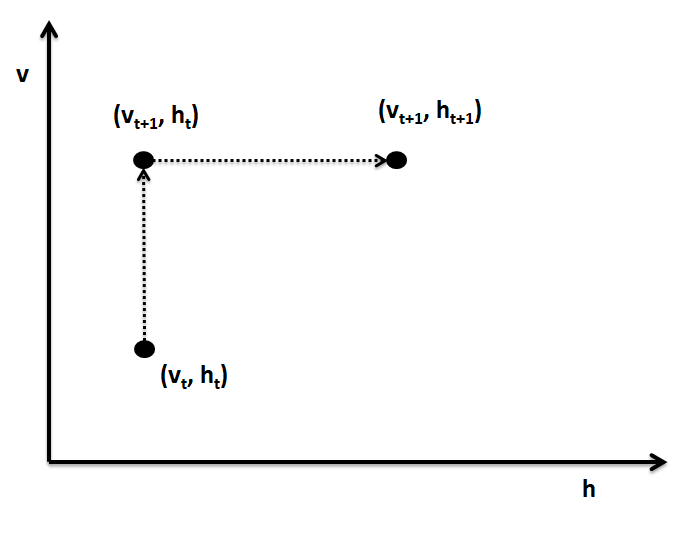
\includegraphics[width=0.6\textwidth]{pics_sdbn/gibbs.png}
	\caption{Gibbs sampling on RBM.}
	\label{fig:gibbs}
\end{figure}
The second term is perfect fit for Gibbs sampling, since we can $ p(\mathbf{v}, \mathbf{h} \mid \Theta) $ as a 2D vector and generating the samples by jumping in a Markov Chain with the transformation probability matrix $ p(\mathbf{v} \mid \mathbf{h}, \Theta) $ and $ p(\mathbf{h} \mid \mathbf{v}, \Theta) $, see Figure~\ref{fig:gibbs} and Section~\ref{sec:Gibbs}.
So, with the given data $ \mathbf{v}_0 $ and the sampling data $ \mathbf{h}_0 $, we have the initial data point in this Markov Chain,  ($ \mathbf{v}_0, \mathbf{h}_0$).
The transformation starts from the axis of $ \mathbf{v} $, then we get $ \mathbf{v}_1 \sim p( \mathbf{v} \mid \mathbf{h}_0, \Theta) $.
It follows the next axis $ \mathbf{h} $, similarly we get $ \mathbf{h}_1 \sim p( \mathbf{h} \mid \mathbf{v}_1, \Theta) $.
So far we obtain the first sample along the Markov Chain, ($ \mathbf{v}_1, \mathbf{h}_1$) thus to solve the objective function with one iteration.
The algorithm is described below:   
\begin{algorithm}[h]
	\caption{Learning on RBM Parameters with $ CD_1 $}
	\label{alg:learn}
	\begin{algorithmic}
		%			\State Initialisation $\mathbf{x}_0 = [x_0(1),x_0(2),...,x_0(M)]$,  \Comment{Random initialise $\mathbf{x}_0$}
		\For{$t=1, 2, ..., K$} \Comment{K number of training data $ \mathbf{V} $, 1 data each iteration}
		%			\For{$k=1, 2, ..., M$}
		\State $ \mathbf{h}_t \sim p( \mathbf{h} \mid \mathbf{v}_t, \Theta) $
		\Comment{Generate $ \mathbf{h}_t $ given $ \mathbf{v}_t $ }
		\State $ \mathbf{v}_{t+1} \sim p( \mathbf{v} \mid \mathbf{h}_{t}, \Theta) $
		\Comment{Generate $ \mathbf{v}_{t+1} $ on v axis using Gibbs sampling }
		\State $ \mathbf{h}_{t+1} \sim p( \mathbf{h} \mid \mathbf{v}_{t+1}, \Theta) $
		\Comment{Generate $ \mathbf{h}_{t+1} $ on h axis using Gibbs sampling }
		\State $ \dfrac{\partial \hat{l} (\Theta \mid \mathbf{D})}{\partial W_{ij}} = v_{t,i} h_{t,j} - v_{t+1,i} h_{t+1,j}$
		\State $ \dfrac{\partial \hat{l} (\Theta \mid \mathbf{D})}{\partial a_{i}} = v_{t,i} - v_{t+1,i} $
		\State $  \dfrac{\partial \hat{l} (\Theta \mid \mathbf{D})}{\partial b_{j}} = h_{t,j} - h_{t+1,j}$
		\State $ \Delta W_{ij} = \eta ( v_{t,i} h_{t,j} - v_{t+1,i} h_{t+1,j}) $
		\Comment{Update $ W_{ij} $}
		\State $ \Delta a_{i} = \eta ( v_{t,i} - v_{t+1,i}) $
		\Comment{Update $ a_{i} $}
		\State $ \Delta b_{j} = \eta ( h_{t,j} - h_{t+1,j}) $
		\Comment{Update $ b_{j} $}
		%			\EndFor
		\EndFor
	\end{algorithmic}
\end{algorithm}

